\clearpage


\section{Studies of Jets from Pileup}
\label{sec:pujets}

In order to ensure the jets which pass the jet selection are from the hard collision rather than from pileup (PU), we will use MC truth information to define a method in which we can distinguish between these jets.

The following dataset is used:

\begin{itemize}
\scriptsize
\item \verb=/DYJetsToLL_M-50_TuneZ2Star_8TeV-madgraph-tarball/Summer12_DR53X-PU_S10_START53_V7A-v1/AODSIM=
\end{itemize}

\subsection{Selection}
The preselection requirements from the inclusive analysis are used to study the PU jets, specifically:

\begin{itemize}
\item Require two leptons which both pass the lepton selection with \pt $>$ 20 \GeVc 
\item 81 GeV $<$ \mll $<$ 101 GeV
\item Require at least two jets both with \pt $> 30$ \GeVc~and $|\eta| < 2.5$ 
\end{itemize}

\subsection{Defining Jets to be ``Matched'' to Genjets}
In order to determine which jets are from the hard collision and which jets come from PU using the MC truth information, the $\Delta$R between each pfjet and the closest status 1 generator level jet with \pt $>$ 20 \GeVc is calculated. By examining the distribution in Fig. \ref{fig:dralljets} we choose a cut value of $\Delta$R $<$ 0.4 to define our jets as ``matched'' to a genjet, and if $Delta$R $>$ 0.4, then the jet is defined to be a PU jet.

%% dr of all jets plot
\begin{figure}[!h]
\begin{center}
\begin{tabular}{cc}
%% 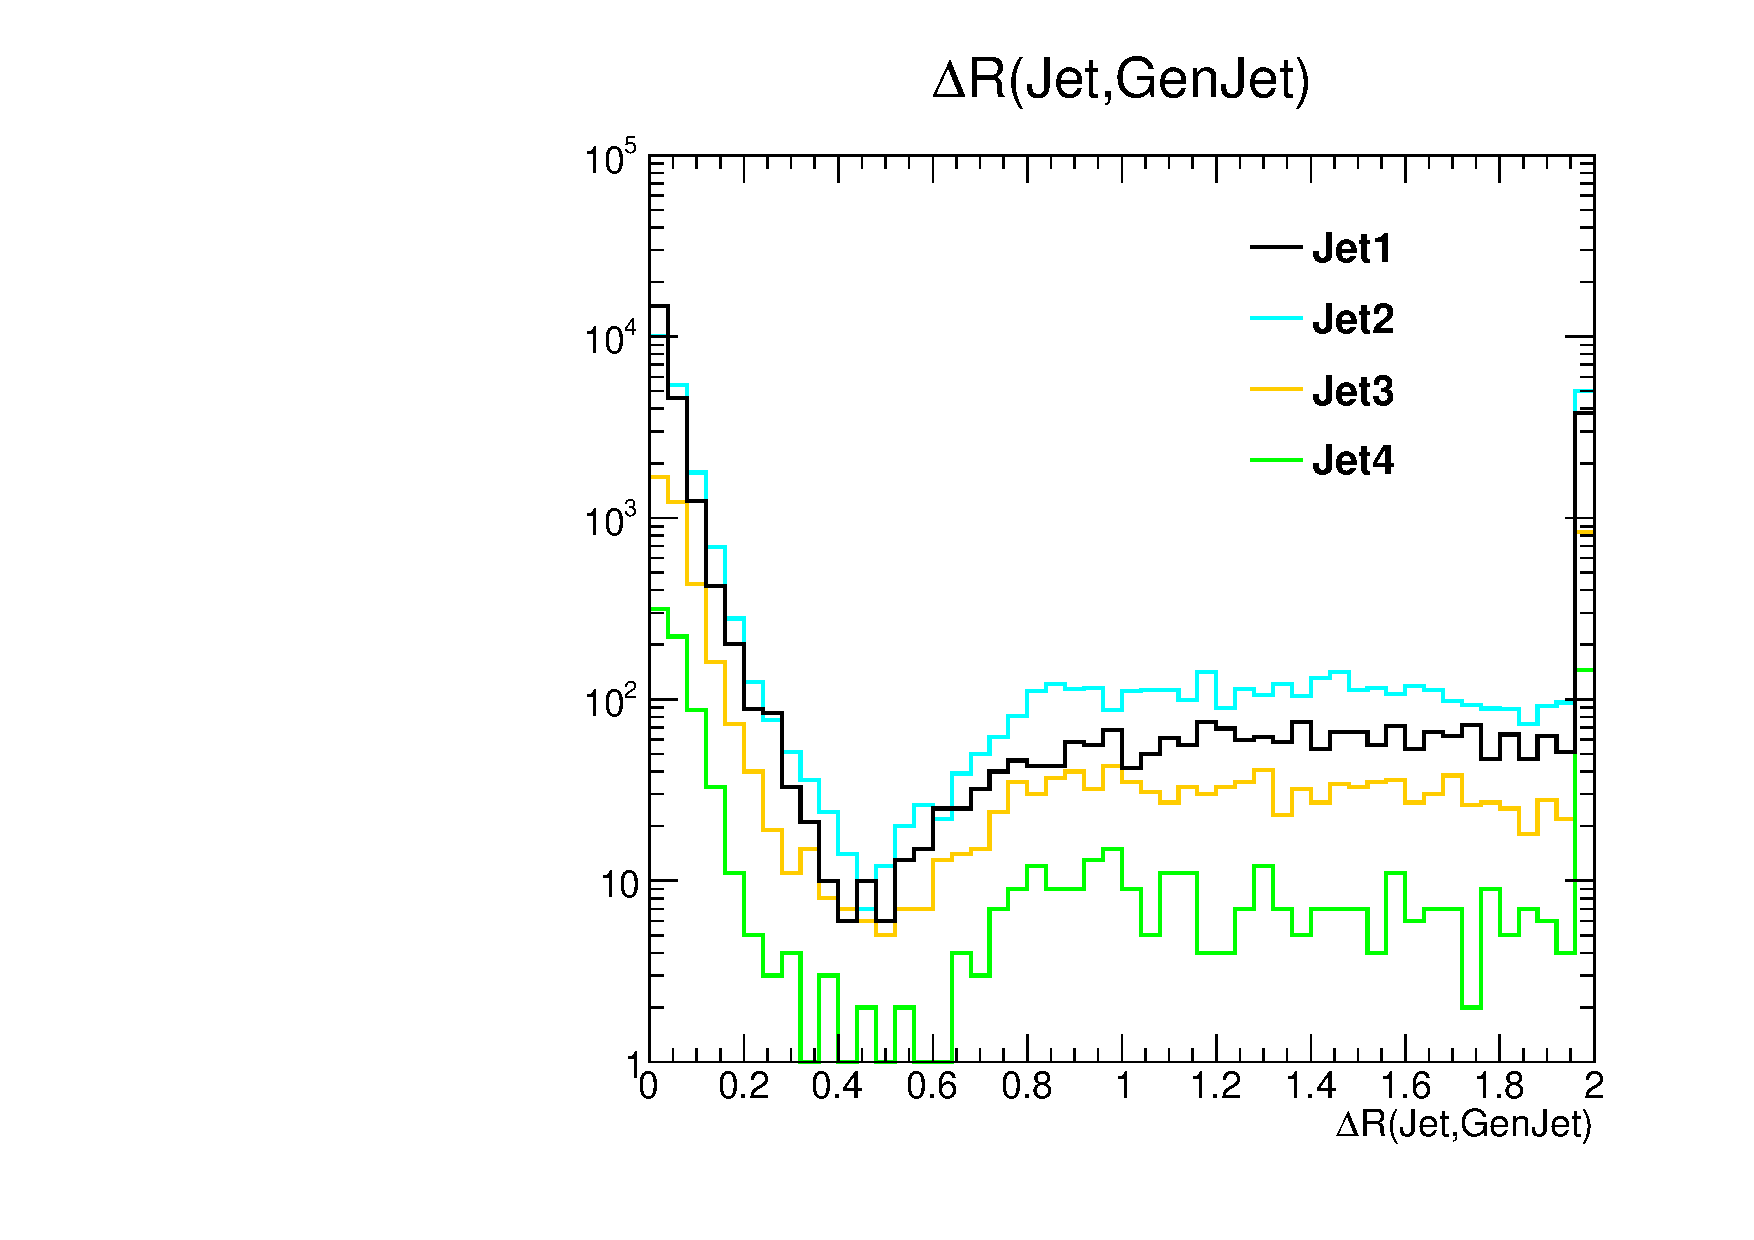
\includegraphics[width=0.6\textwidth]{/home/users/cwelke/public_html/Zmet/jetstudy/pdf/jetAlldrgen_Inclusive_Selection.pdf}
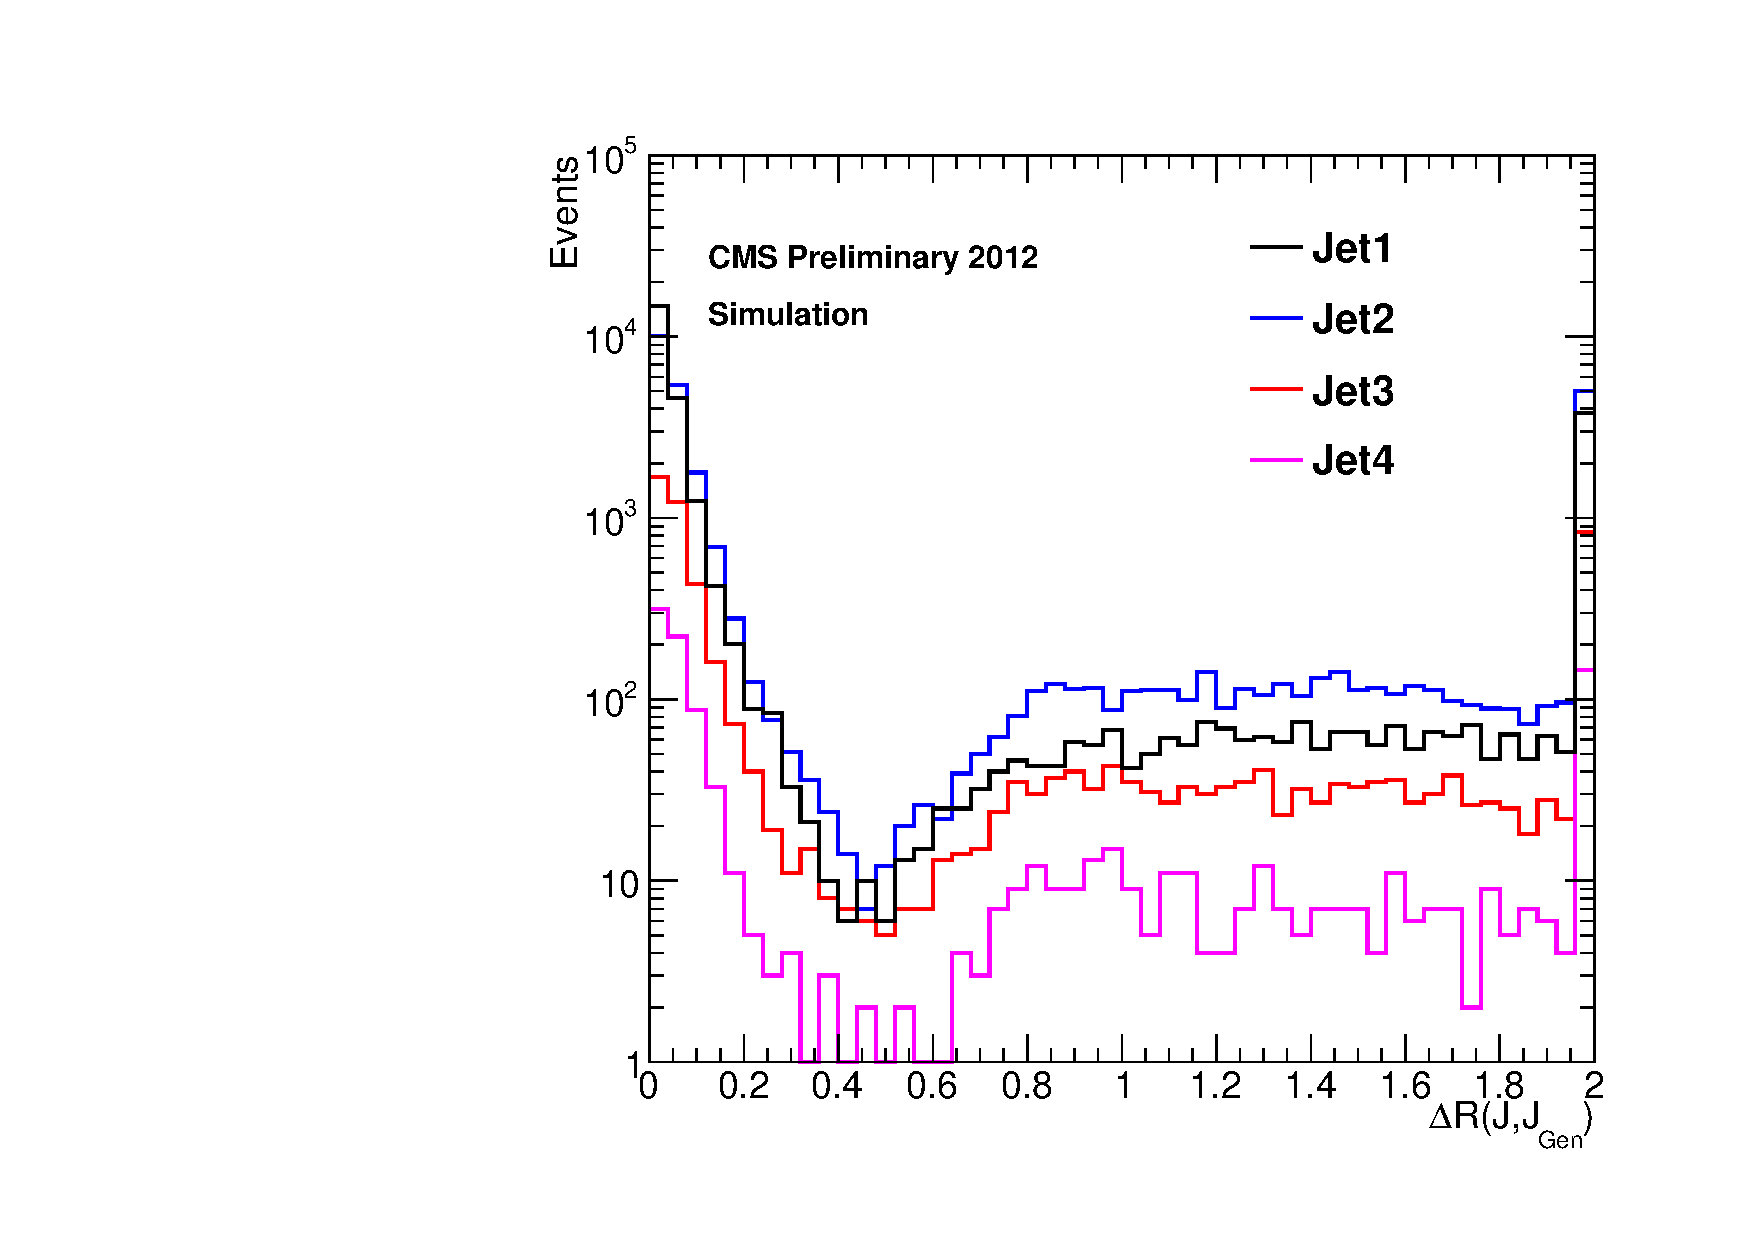
\includegraphics[width=0.6\textwidth]{plots/dralljets.pdf}
\end{tabular}
\caption{The $\Delta$R for the four highest \pt jets is shown. We are using $\Delta$R $<$ 0.4 to define jets to be ``matched'' to a genjet.
\label{fig:dralljets}
}
\end{center}
\end{figure}

\subsection{Defining $\beta$}
Now that we've established how to distinguish between PU jets versus hard scatter jets using MC truth information, we want to be able to be able to make the same distinction in data (without the truth information). In order to do this, the variable $\beta$ is defined for each jet in equation (\ref{eqn:beta}) 

\begin{equation}
\beta = \frac{\sum_i({track~p_T^i})^2_{tracks~with~dz~>~0.5~cm}}{\sum_i ({track~p_T^i})^2_{All~Tracks}}
\label{eqn:beta}
\end{equation}

Jets with $\beta$ close to 1 are jets from the hard collision, whereas Jets with $\beta$ close to 0 are PU jets. By looking at the $\beta$ distribution of the two highest \pt jets in Figure.~\ref{fig:jetbeta}, we choose a cut value of $\beta$ $>$ 0.2 to remove PU jets. 

%% The plots in Fig.~\ref{fig:jetbeta} show the $\beta$ distributions for the two highest \pt jets after being seperated as PU jets and hard scatter jets.

%% jet beta plots
\begin{figure}[!hbtp]
\centering
\subfigure[]{
\centering
\label{subfig:jet1beta}
%% \includegraphics[width=.4\textwidth]{/home/users/cwelke/public_html/Zmet/jetstudy/pdf/jet1beta2_05.pdf}
\includegraphics[width=.4\textwidth]{plots/jet1beta2_05.pdf}
}
\subfigure[]{
\centering
\label{subfig:jet2beta}
%% \includegraphics[width=.4\textwidth]{/home/users/cwelke/public_html/Zmet/jetstudy/pdf/jet2beta2_05.pdf}
\includegraphics[width=.4\textwidth]{plots/jet2beta2_05.pdf}
}\\
\caption{$\beta$ for jet1 \subref{subfig:jet1beta} and jet2 \subref{subfig:jet2beta}.}
\label{fig:jetbeta}
\end{figure}

We list the efficiencies for the $\beta$ cut in table \ref{table:efficiency}

\begin{table}[htb]
\begin{center}
\caption{\label{table:efficiency} Selection efficiencies for a cut value of $\beta > 0.2$. }
\begin{tabular}{l|cc}
\hline
\hline
$\beta > 0.2$ & PU Jets & Hard Scatter Jets \\
\hline
Jet 1 & 12\% & 99\% \\
Jet 2 & 17\% & 99\% \\
\hline
\hline
\end{tabular}
\end{center}
\end{table}

\subsection{Dilepton \pt}
These plots show the dilepton mass of events which pass the inclusive analysis selection. As you can see in Fig.~\ref{fig:dileppt}, the PU jets have a significant contribution to the shape of the distribution at low \pt. The rejection of PU jets leads to a dilepton \pt distribution which looks healthy (i.e. the double peak structure is gone). 

%% dilepton Pt Plots
\begin{figure}[!hbtp]
\centering
\subfigure[]{
\centering
\label{subfig:jet1cut}
%% \includegraphics[width=.4\textwidth]{/home/users/cwelke/public_html/Zmet/jetstudy/pdf/dilep_Pt_jet1_drgen_Selection.pdf}
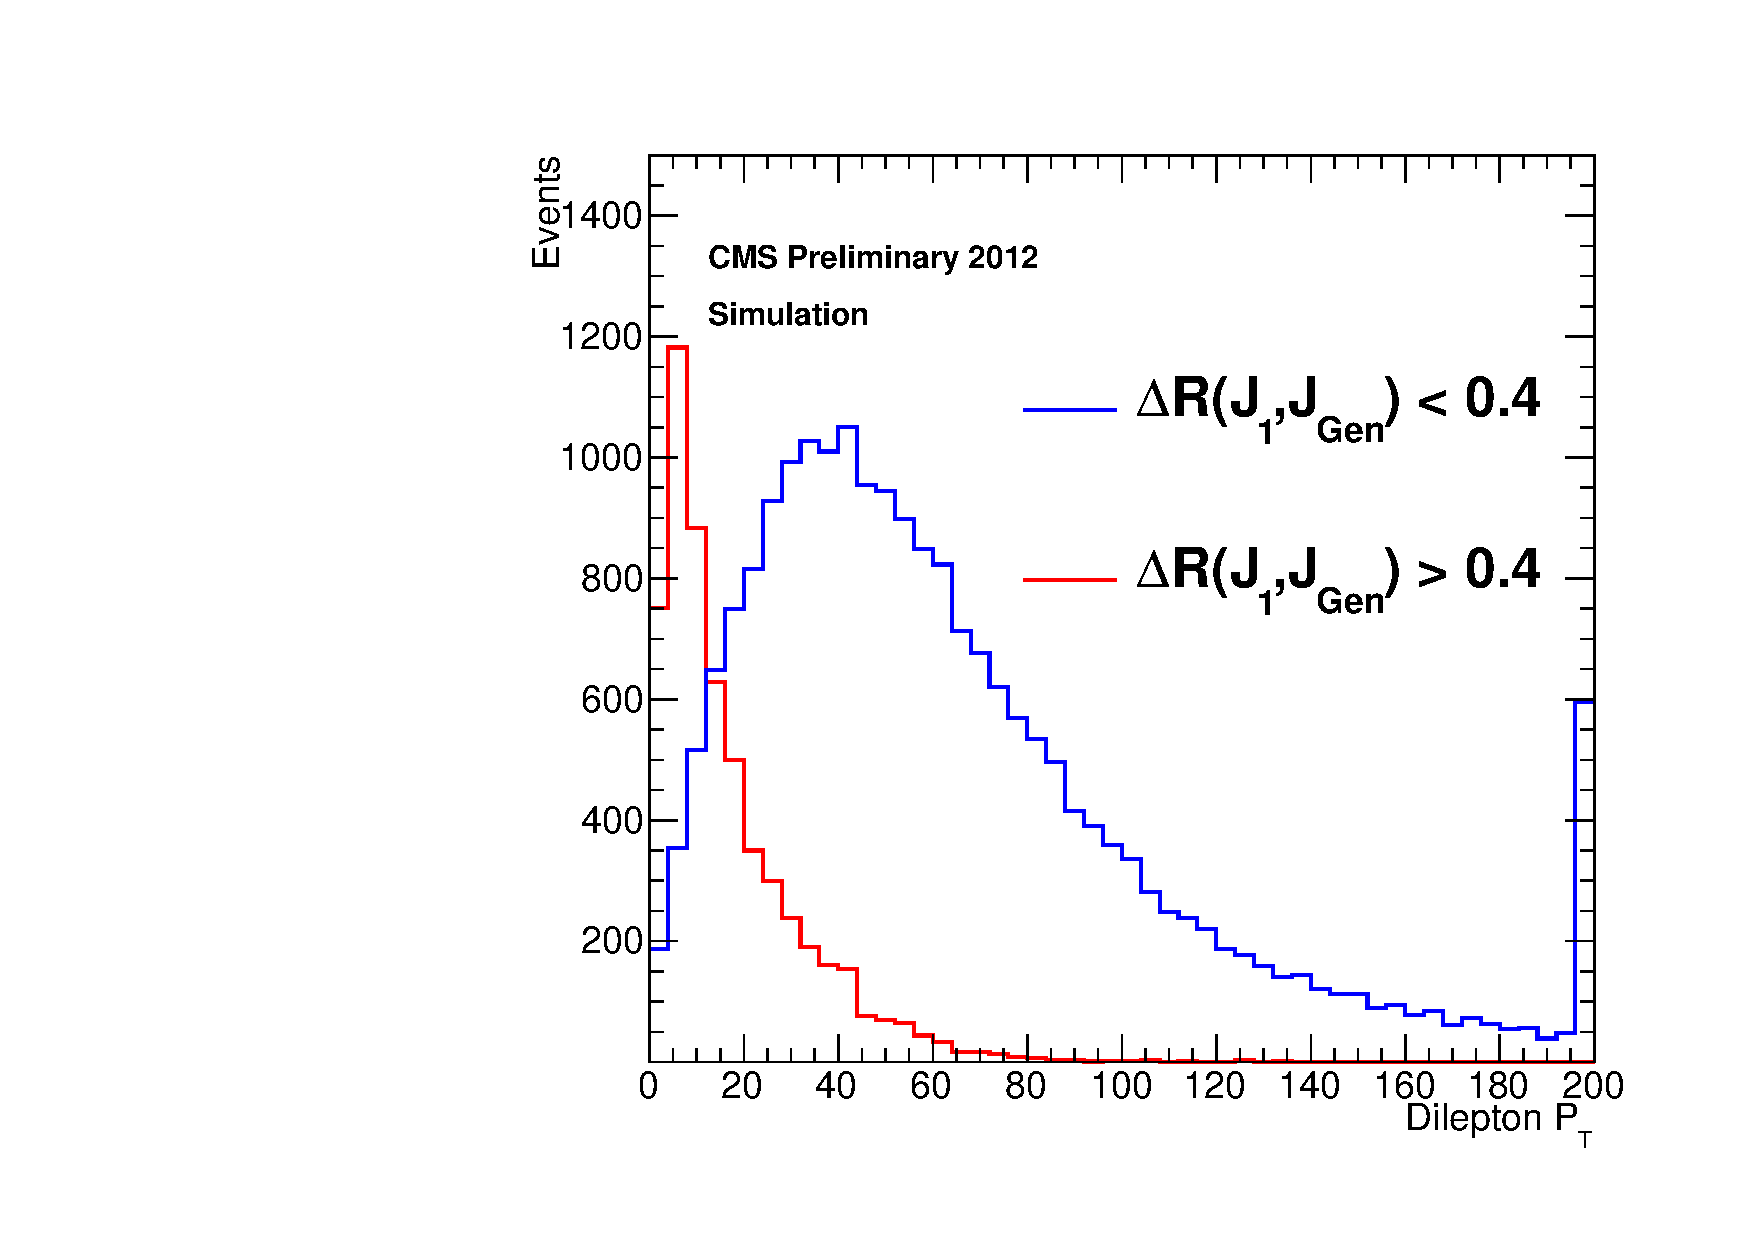
\includegraphics[width=.4\textwidth]{plots/dilep_pt_jet1.pdf}
}
\subfigure[]{
\centering
\label{subfig:jet12cut}
%% \includegraphics[width=.4\textwidth]{/home/users/cwelke/public_html/Zmet/jetstudy/pdf/dilep_Pt_jet1_jet2_drgen_Selection.pdf}
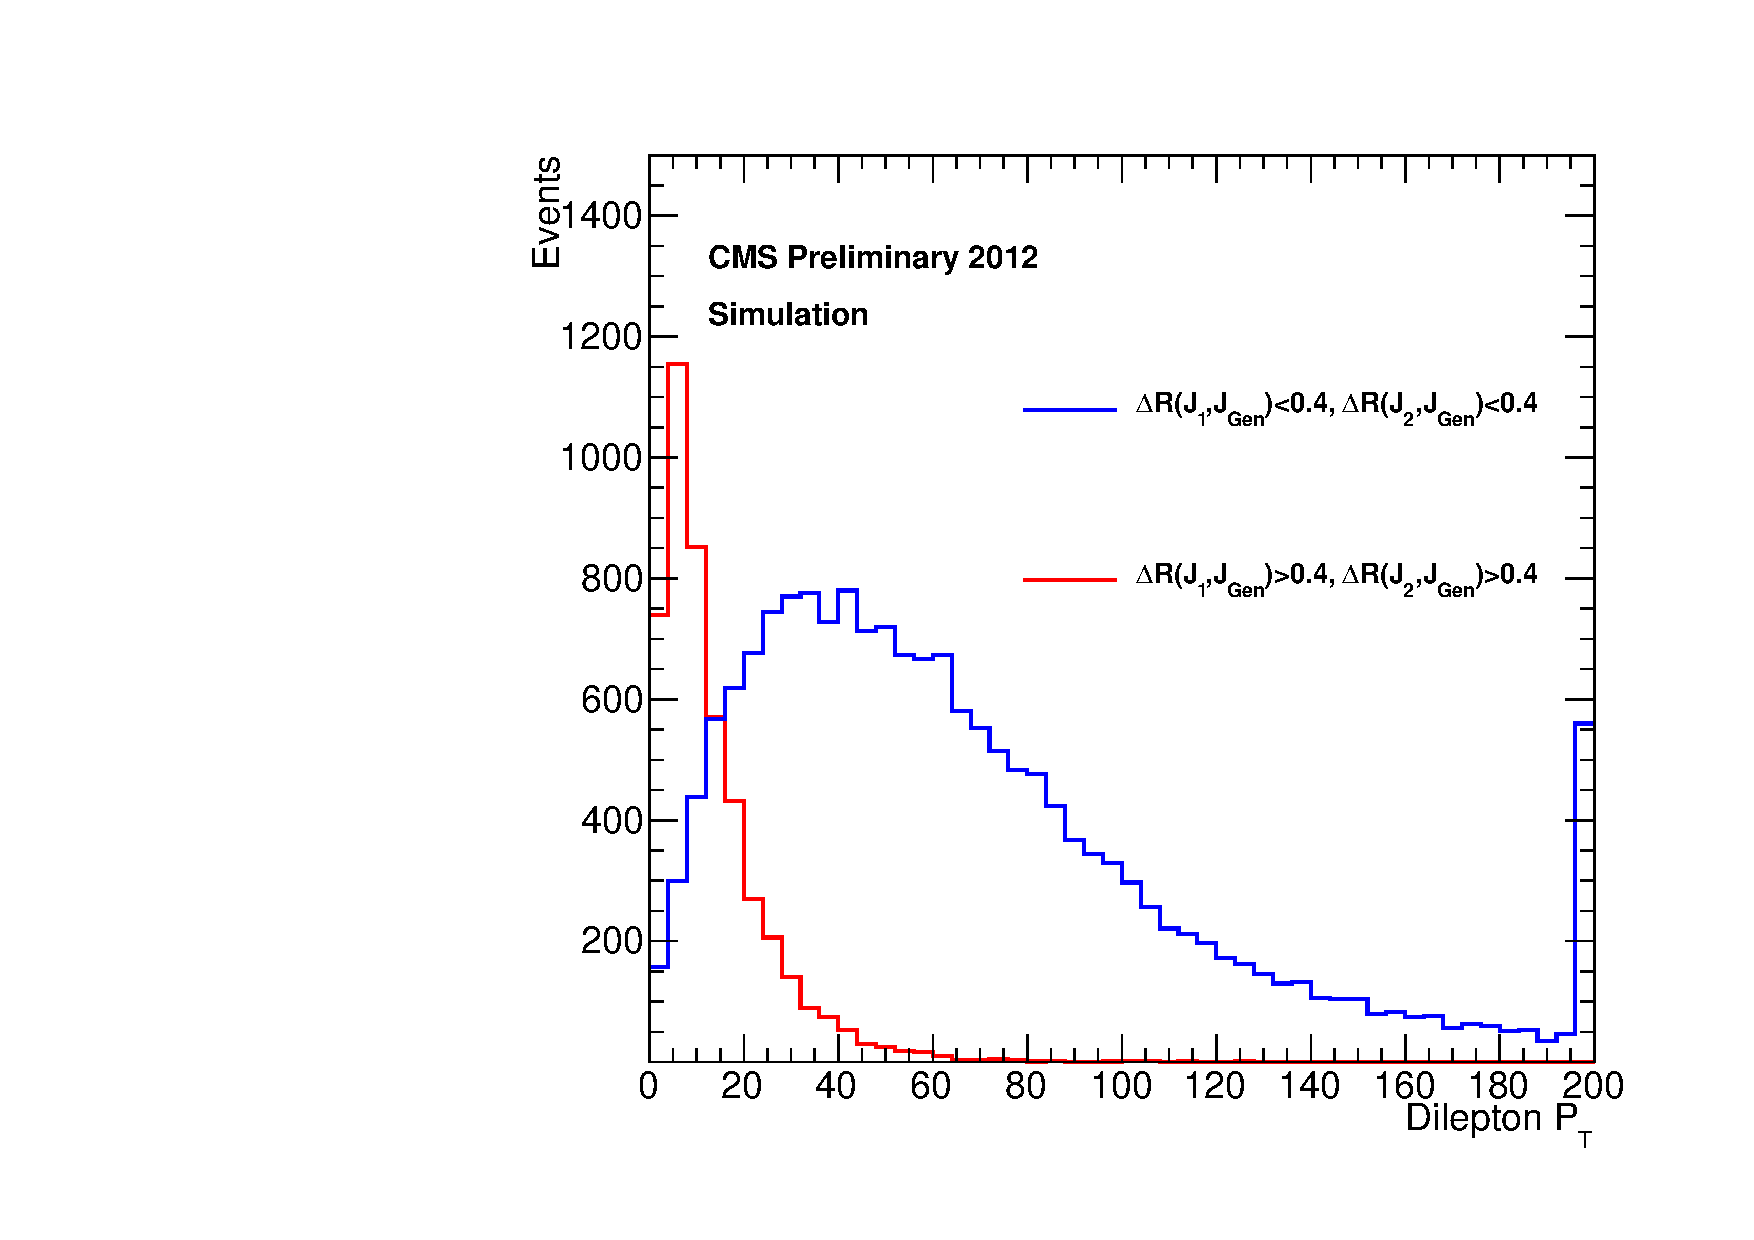
\includegraphics[width=.4\textwidth]{plots/dilep_pt_jet1_jet2.pdf}
}\\
\caption{Dilepton \pt with $\Delta$R cut on jet1 \subref{subfig:jet1cut} and $\Delta$R cut on jet1 and jet2 \subref{subfig:jet12cut}.}
\label{fig:dileppt}
\end{figure}


\subsection{Distinguishing Event Type}
If we seperate the jets in the event by jet type (i.e. PU jets vs hard scatter jets), we can determine what type of event we are looking at. The possible event types are \z + 2 hard scatter jets, \z + 1 hard scatter jet and 1 PU jet, and \z + 2 PU jets. 
In Fig.~\ref{fig:2Ddrplot}, the $\Delta$R between the highest \pt jet and its associated gen jet is plotted against the $\Delta$R between the second highest \pt jet and its associated gen jet. We can use this plot to visually see the various regions which contain the three different event types.

%% dr of all jets plot
\begin{figure}[!h]
\begin{center}
\begin{tabular}{cc}
%% \includegraphics[width=0.6\textwidth]{/home/users/cwelke/public_html/Zmet/jetstudy/pdf/2D_drgen_Selection.pdf}
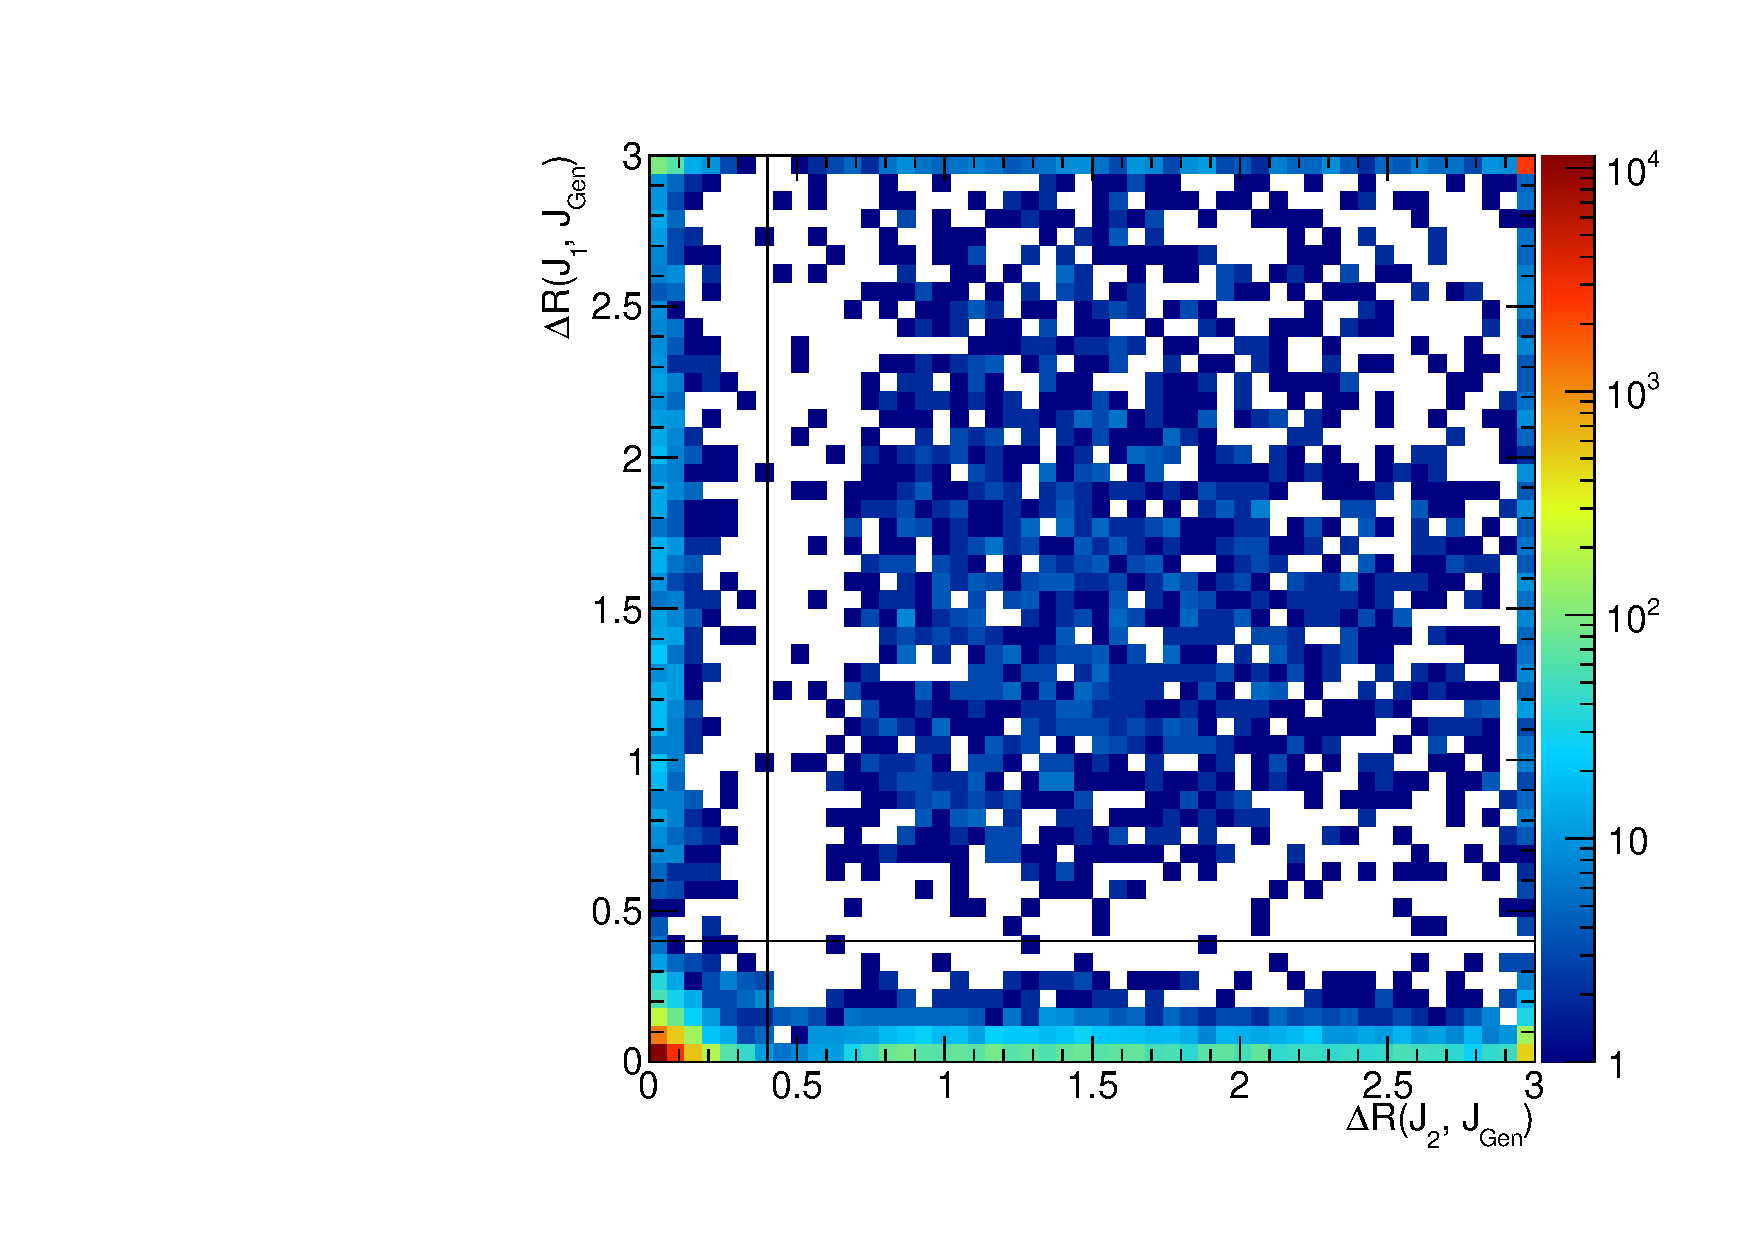
\includegraphics[width=0.6\textwidth]{plots/2D_drgen.pdf}
\end{tabular}
\caption{The $\Delta$R(jet1, genjet) vs. $\Delta$R(jet2, genjet)
\label{fig:2Ddrplot}
}
\end{center}
\end{figure}

We label the sections on this plot starting from the top left and going clockwise as sections 1 through 4. The events with 2 hard scatter jets are represented in section 4, the section with 1 hard scatter jet and 1 PU jet are represented in sections 1 and 3, adn the events with 2 PU jets are represented in section 2. Now we will look at $\Delta\phi$ between the 2 lead jets to see if we can better understand the events.

\subsection{$\Delta\phi$ Between the Two Jets}
In Fig.~\ref{fig:dphiplots}, we show the distribution of the $\Delta\phi$ between the two highest pt jets in the event. 

%% delta phi plots
\begin{figure}[!hbtp]
\centering
\subfigure[]{
\centering
\label{subfig:dphisamecut}
%% \includegraphics[width=.4\textwidth]{/home/users/cwelke/public_html/Zmet/jetstudy/pdf/dphij1j2_jet1_jet2drgen_Selection.pdf}
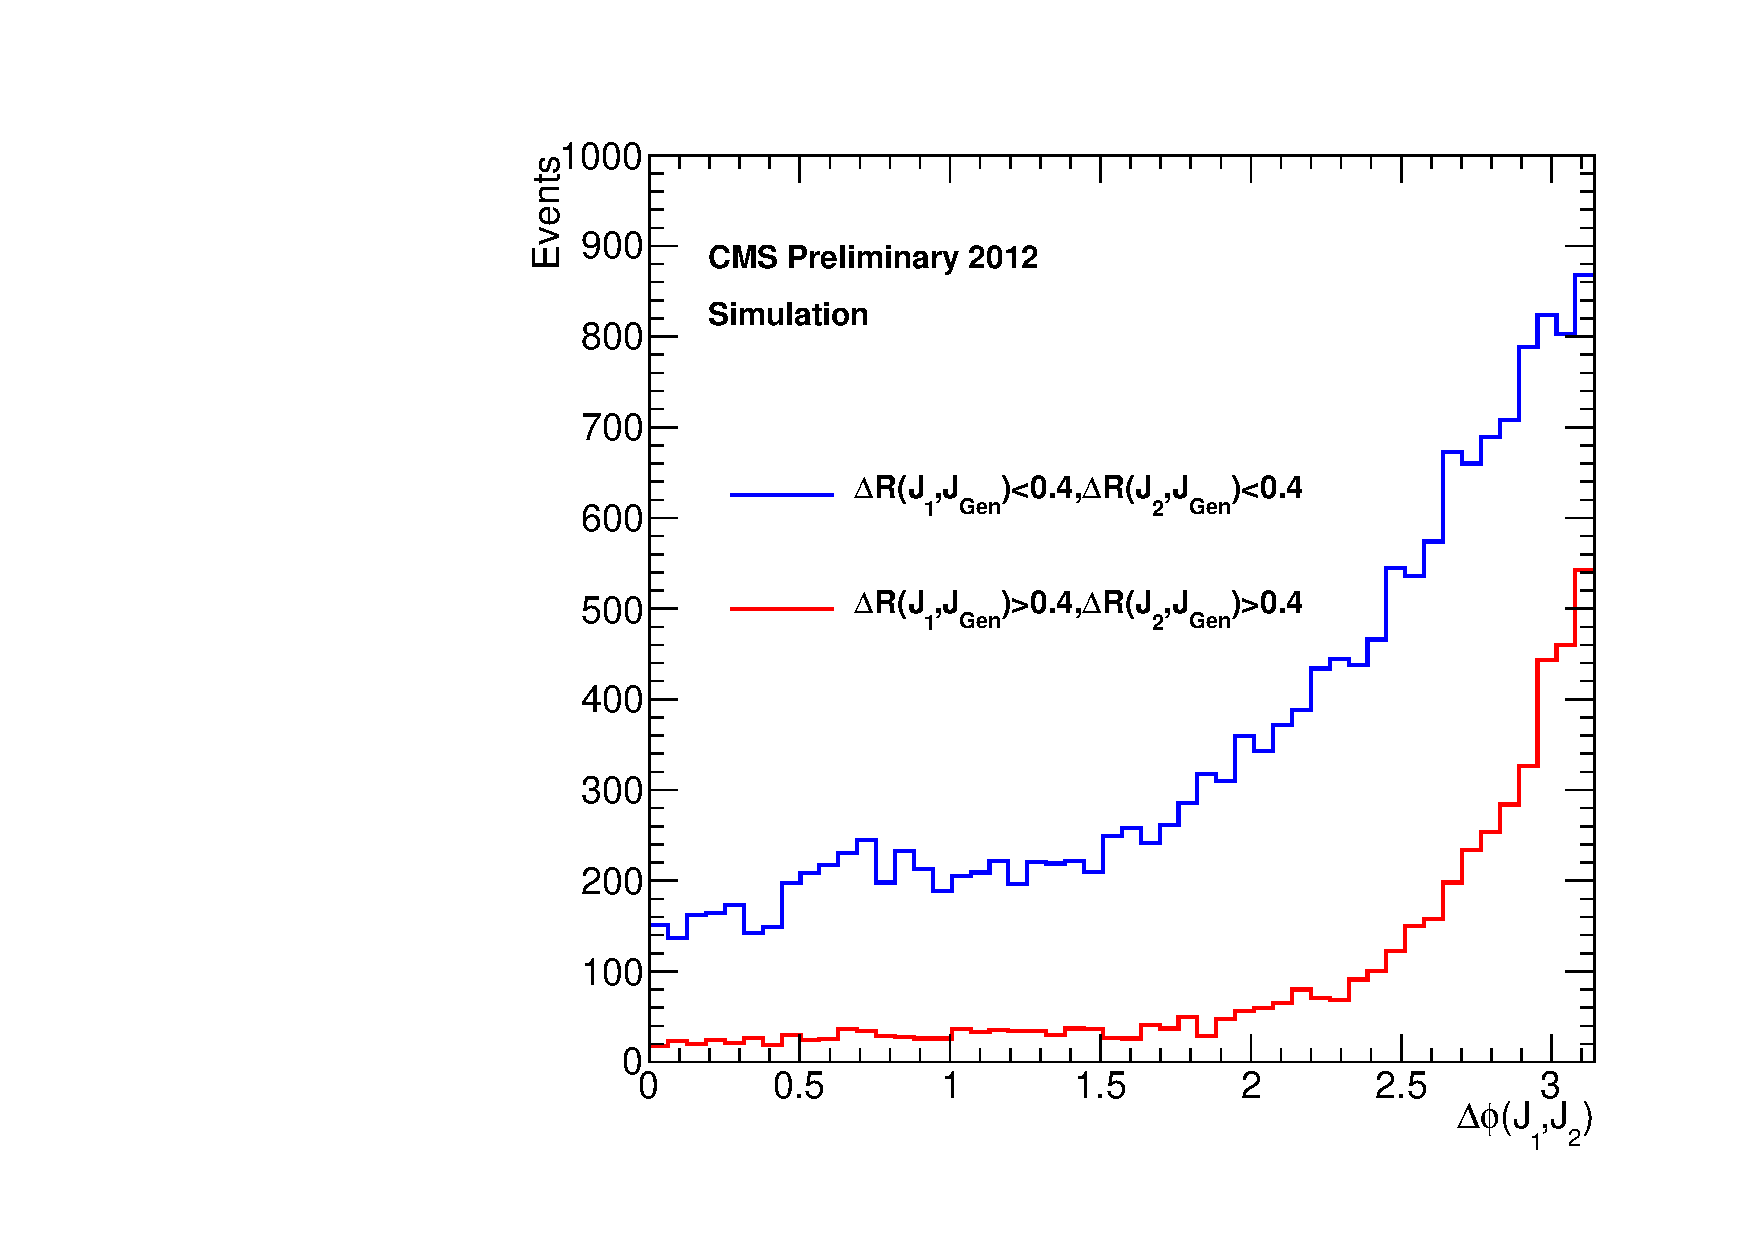
\includegraphics[width=.4\textwidth]{plots/dphi_jet1_jet2.pdf}
}
\subfigure[]{
\centering
\label{subfig:dphianticut}
%% \includegraphics[width=.4\textwidth]{/home/users/cwelke/public_html/Zmet/jetstudy/pdf/dphij1j2_All_Selection.pdf}
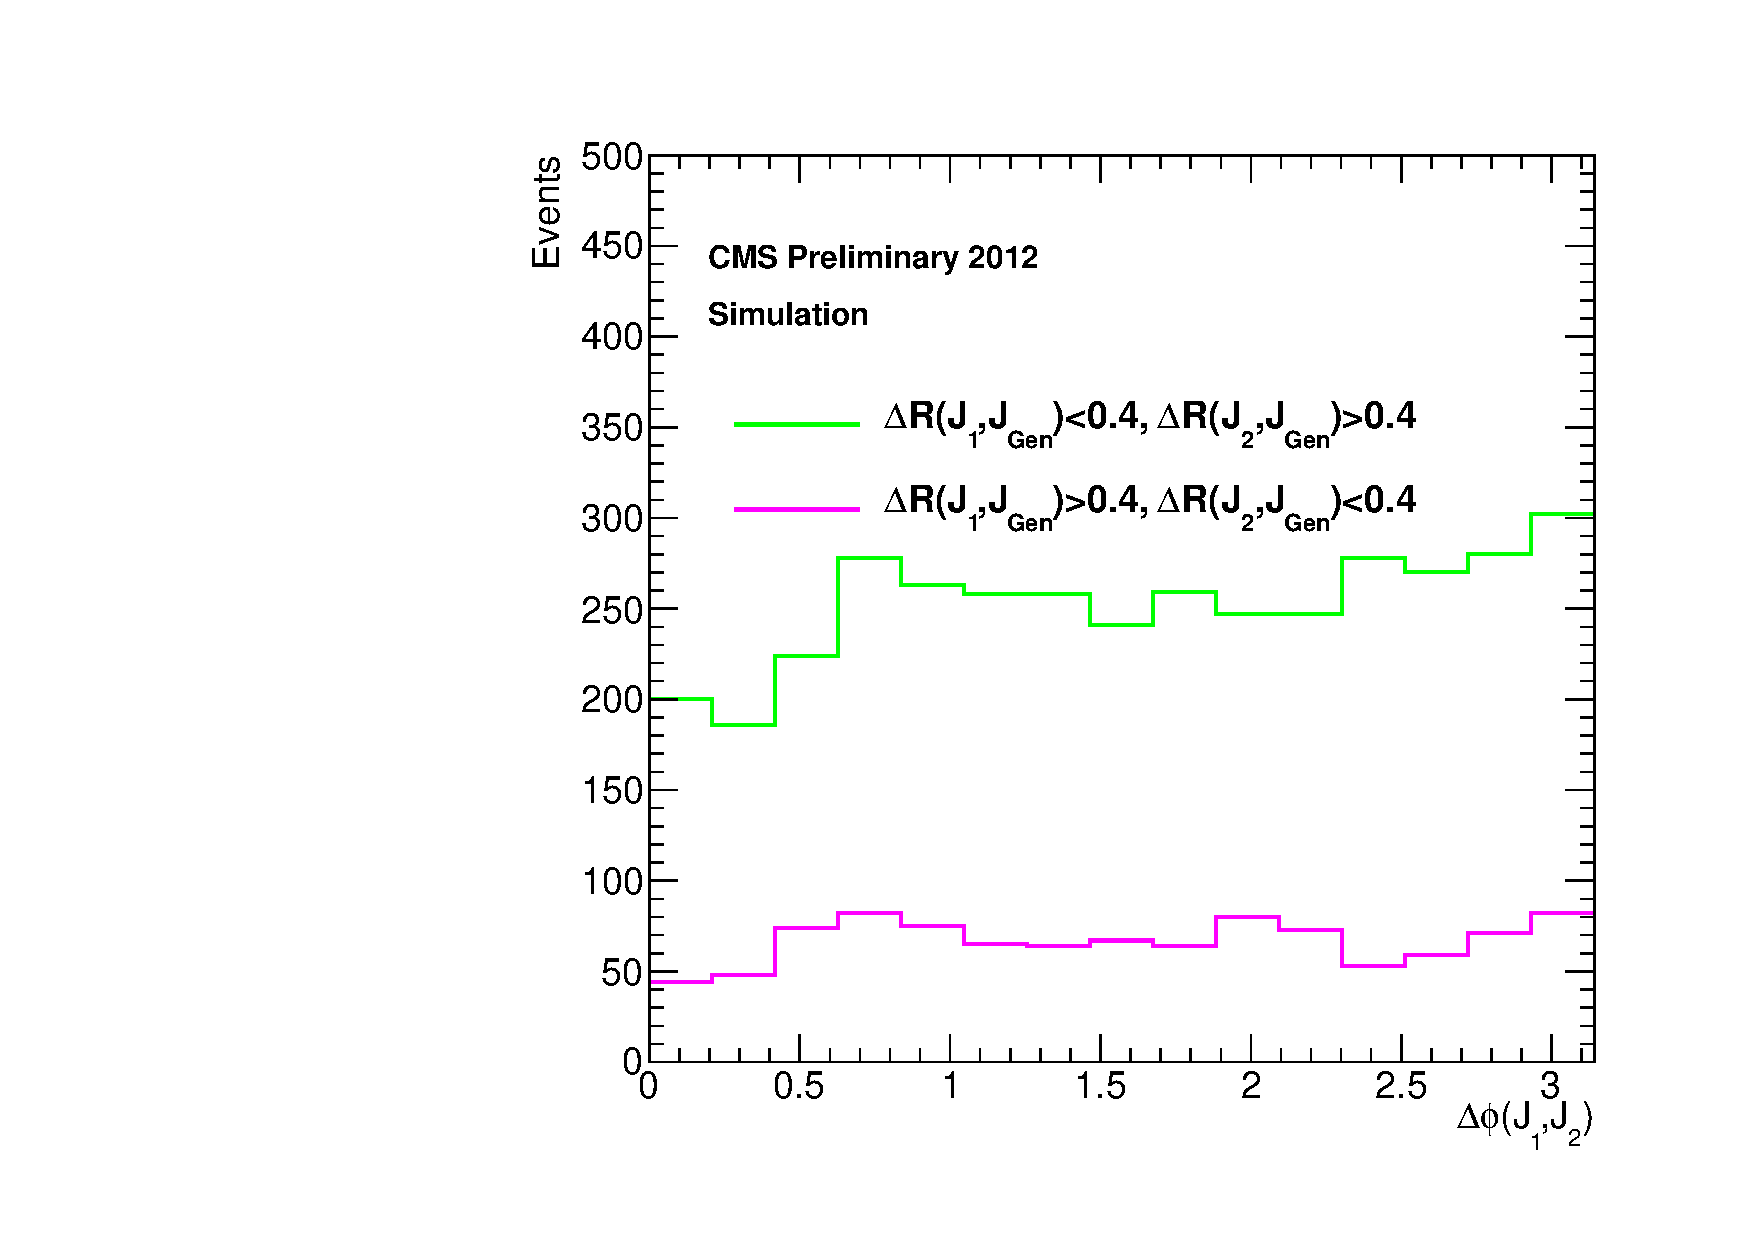
\includegraphics[width=.4\textwidth]{plots/dphi_jet1_antijet2.pdf}
}\\
\caption{The $\Delta\phi$ distribution between the two leading jets is shown in blue where both jets are matched to gen jets and shown in red for events where both jets are from PU in \subref{subfig:dphisamecut} and in \subref{subfig:jet12cut} one jet is matched to a gen jet and the other jet is not matched to a gen jet.}
\label{fig:dphiplots}
\end{figure}

These distributions represent the various sections in Fig.~\ref{fig:2Ddrplot} as follows, section 1 is magenta, section 2 is red, section 3 is green, and section 4 is blue. 
The events in section 2 show a strong correlation for events to be back to back. The events in sections 1 and 3 show a flat distribution which implies that the jets $\phi$ is uncorrelated. 

\clearpage
